% !TEX root = ../thesis_main.tex

\section{Validation of \pygbe and Replication of Ellis et al. 2016  et al 2005} \label{sec:rep_val_ellis}
\graphicspath{{replication_validation/figs/}}

The work of Ellis et al. "Aspect-ratio driven evolution of high-order resonant modes and near-field distributions in
localized surface phonon polariton nanostructures." \cite{ellis2016} has both computational and experimental results, which makes 
it a perfect candidate to perform a validation as well as a replication study. Ellis and coworkers studied the excitation of 
multipolar localized surface polaritons (SPhP) by computing and measuring the polarized reflectance on 4H-SiC pillars of
fixed width ($W = 400$ nm), fixed height ($H=950$ nm) and varied length ($L=400-4800$ nm). To reduce coupling these pillars are 
pattern on a square grid with $P = L + 500$ nm. In their experiments (simulations), they measure (compute) the polarized reflectance
with the incident polarization oriented parallel or perpendicular to the length ($L$) of the pillars. We started by replicating a 
computational result shown in Figure S4 of their supplementary material. Figure S4 of the 
supplementary material shows simulation results for the resonance spectral position of the lower frequency mode when the angle of 
incidence is $22$ degrees and the polarization is parallel to the length of the pillars. They present results for separations of $500$ nm 
(red curve) and $5000$ (black curve), the latter a good candidate for replication with \pygbe because a larger gap diminishes 
the coupling (not included in our model). The setup in our computations consists of a single pillar with no substrate.
Secondly, we aimed to replicate the results of Figure 2a of the main paper, 
corresponding to reflectance measurements across the wave number for pillars of aspect ratio $AR=4$, angle of incidence 22 degrees, 
and incoming parallel polarization. For this case the authors also reported experimental results and we used them for the 
validation of our solver. For all the simulations involved in the replication and validation studies we use experimental values of the 
complex dielectric data for 4H-SIC provided by the authors of Ellis et al. via private communication. 

\textbf{Differences in method and input data}

\begin{itemize}

\item {The simulations of Ellis et al. compute the solution of Maxwell's equations using the RF package
of the finite element solver in the commercial software COMSOL. Their setup consists of one pillar over a 
substrate, with periodic boundary conditions to emulate the array of pillars used in their experiments. In our 
solver we use the boundary element method in the quasistatic approximation, which is suitable since the wavelengths
involved are in the range $10000-12500$ nm, and are considerably larger than the pillar's dimensions. We computed 
the extinction cross section, where the resonance expresses as peaks instead of dips as in the reflection plots of 
Ellis et al. The intensity of the peaks is not comparable; however, we are looking to match the wave number at which
they happen.}

\item {The simulations of Ellis et al. rely on a volumetric model and use a volumetric mesh. In our 
solver, the geometries are represented as triangular surface meshes. For the validation and replication of Figure 2a of 
their paper, where the pillars have an aspect ratio of $AR=4$, we used a non-uniform triangular mesh ($N=4398$) that 
was provided by the authors of Ellis et al. However, for the replication of the results in Figure S4 of the supplementary material, 
we were missing the remaining meshes for the other aspect ratios. To overcome this, we generated the meshes with our Python 
script, and we determined the density to be used by comparing simulations for the case of aspect ratio $AR=4$ with our mesh and 
the one provided by Ellis and coworkers. Using approximately double the number of elements ($N=8564$) than the original mesh 
and rounding the edges using Trimesh, the relative errors for the extinction cross-section were, on average, smaller than 
$3\%$, and the variations on the wave number of the peak position was smaller than $1$ cm$^{-1}$. After this analysis we 
decided on a density of $\approx \; 1.7 \times10^{-5}$ triangles per $\text{\AA}$ squared, which we used to create the meshes
for the remaining aspect ratio geometries.}

\item {In Ellis et al. they perform simulations for different angles of incidence of the illuminating vector. To achieve this 
using \pygbe we rotated the geometry, since the direction of the illuminating vector in our solver is fixed.}
\end{itemize}

\subsection{Replication of Figure S4 of supplementary material of Ellis et al. 2016}

To replicate Figure S4 of the supplementary material we identified the lower-frequency mode for every different 
aspect ratio in our computations. For the values of aspect ratio ($AR$) from 1 to 7, we computed the extinction cross section 
$C_{ext}$ across wave numbers in the range $800-1000$ cm$^{-1}$, and we identified the lower-frequency mode 
($E^{\parallel}_{100}$ for Ellis et al.) that was not a longitudinal mode. The longitudinal modes are the ones associated with 
the height of the pillar and they appear only when we have an angle of incidence that is off-normal. 
Figure \ref{fig:AR_22_vs_norm} shows the results of the extinction cross-section of a SiC pillar for different values of 
length ($L=400$-$2800$ nm), for normal and 22-degrees angle of incidence (see Figure \ref{fig:ellis_ang_inc}). We performed 
the simulations for the long-edge orientation, meaning that the electric field is aligned with the length of the pillar when having a normal 
incidence. From each result of Figure \ref{fig:AR_22_vs_norm}, we selected the lowest non-longitudinal mode and extracted the corresponding wavelength
(see Table \ref{tab:ar_peaks}) to replicate Figure S4 of the supplementary material of Ellis et al. Figure \ref{fig:rep_FS4_ellis} shows the
results from Ellis et al. (obtained using the WebPlotDigitizer) and the results obtained using \pygbe. Table \ref{tab:err_AR} contains the 
percentage error, and we can see that it is below 2$\%$ for all the cases.

\begin{figure}
    \centering
    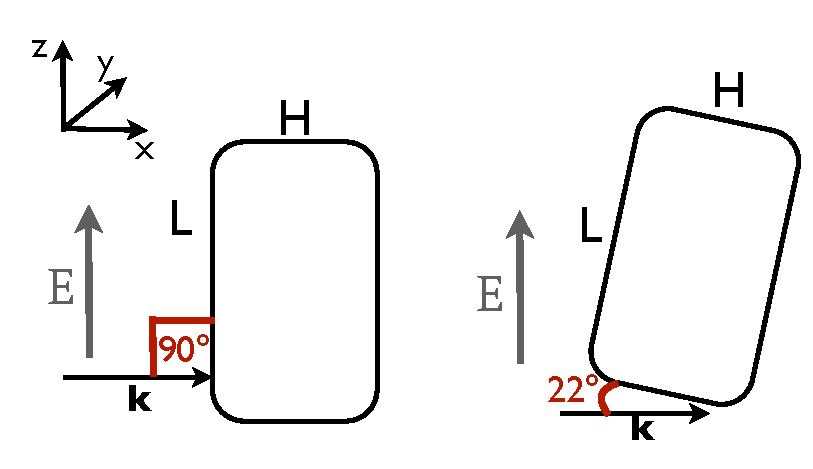
\includegraphics[width=0.45\textwidth]{ellis_ang_inc.pdf} 
    \caption{Diagram showing the angles of incidence in our simulation setups to comply with the configuration in the case from Ellis et al.}
    \label{fig:ellis_ang_inc}
\end{figure}

\begin{figure}
    \centering
    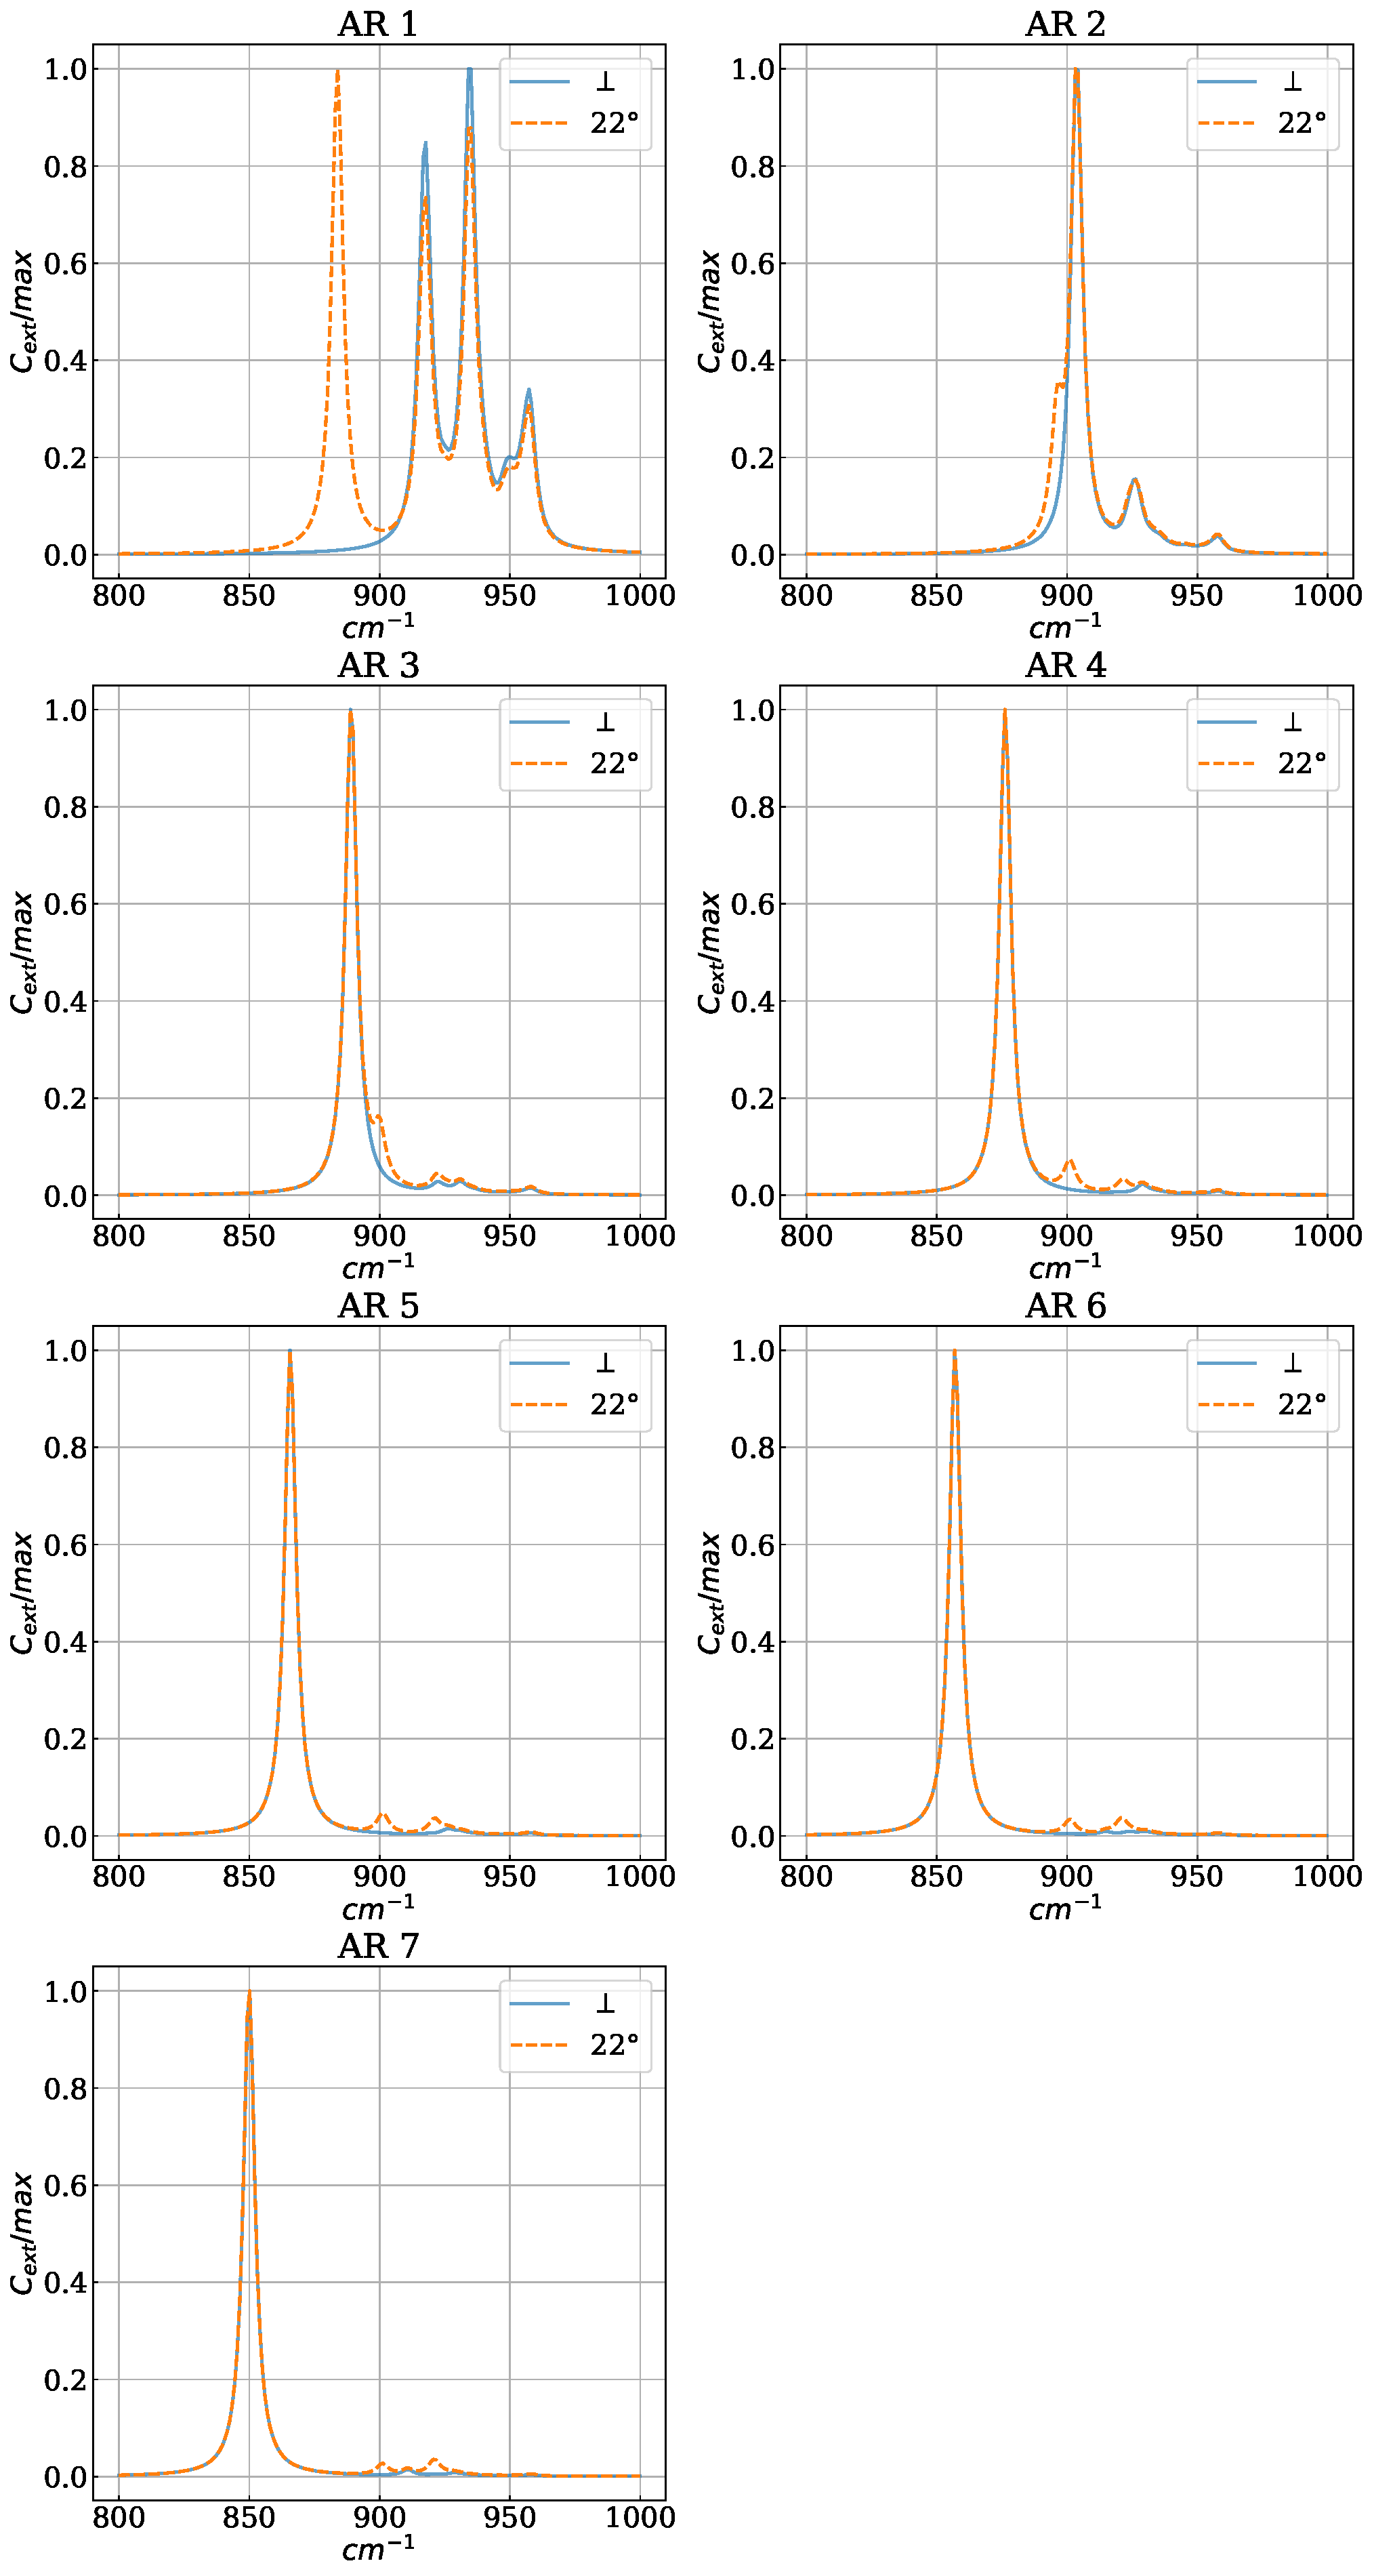
\includegraphics[width=0.72\textwidth]{AR_22_vs_norm.pdf} 
    \caption{Extinction cross-section across wave numbers for SiC pillars of varying aspect ratios,  
             ($H=950$ nm, $W=400$ nm, $L=400$--$2800$ nm, $AR=1$--$7$), with both normal incidence and a 
             22-degree incidence.}
    \label{fig:AR_22_vs_norm}
\end{figure}

\begin{table}
    \centering
      \caption{Wavelength at which peaks happen for different aspect ratios, for runs where the electric
      field is parallel to the length ($L$) of the pillar. We have normal incidence and 22-degree incidence.
      The wavelengths in bold correspond to the lowest mode that is not a longitudinal one.}
      \label{tab:ar_peaks}
      \begin{tabular}{c c c c c c c c}
        \textbf{AR} \\
        \hline
        \multirow{2}{*}{1} & $\perp$ & \textbf{917.73} & 934.092 & 949.604 & 957.325 \\ % <-- Combining 2 rows with arbitrary with (*) and content 12
        & 22$^{\circ}$ & 883.926 & \textbf{917.73} & 935.052 & 949.604 & 957.325 \\ % <-- Content of first column omitted.
        \hline
        \multirow{2}{*}{2} & $\perp$ & \textbf{903.233} & 926.395 & 944.762 & 958.242 \\ % <-- Combining 2 rows with arbitrary with (*) and content 12
        & 22$^{\circ}$ & 896.517 & \textbf{903.233} & 926.395 & 944.762 & 958.242 \\ % <-- Content of first column omitted.
        \hline
        \multirow{2}{*}{3} & $\perp$ & \textbf{888.793} & 922.552 & 931.223 & 948.613 & 958.242 \\ % <-- Combining 2 rows with arbitrary with (*) and content 12
        & 22$^{\circ}$ & \textbf{888.793} & 899.418 & 922.552 & 931.223 & 958.242 \\ % <-- Content of first column omitted.
        \hline
        \multirow{2}{*}{4} & $\perp$ & \textbf{876.186} & 929.32 & 946.639 & 958.242 \\ % <-- Combining 2 rows with arbitrary with (*) and content 12
        & 22$^{\circ}$ & \textbf{876.186} & 901.281 & 921.618 & 929.32 & 945.745 & 958.242 \\ % <-- Content of first column omitted.
        \hline
        \multirow{2}{*}{5} & $\perp$ & \textbf{865.576} & 926.395 & 945.745 & 958.242 \\ % <-- Combining 2 rows with arbitrary with (*) and content 12
        & 22$^{\circ}$ & \textbf{865.576} & 901.281 & 921.618 & 958.242 \\ % <-- Content of first column omitted.
        \hline
        \multirow{2}{*}{6} & $\perp$ &  \textbf{856.904} & 914.793 & 923.489 & 929.32 & 946.639 & 958.242\\ % <-- Combining 2 rows with arbitrary with (*) and content 12
        & 22$^{\circ}$ & \textbf{856.904} & 901.281 & 920.6 & 958.242\\ % <-- Content of first column omitted.
        \hline
        \multirow{2}{*}{7} & $\perp$ &  \textbf{850.134} & 910.963 & 921.618 & 928.372 & 946.639 & 958.242 \\ % <-- Combining 2 rows with arbitrary with (*) and content 12
        & 22$^{\circ}$ & \textbf{850.134} & 901.281 & 910.963 & 920.6 & 958.242\\ % <-- Content of first column omitted.
        \hline
      \end{tabular}
\end{table}

\begin{figure}
    \centering
    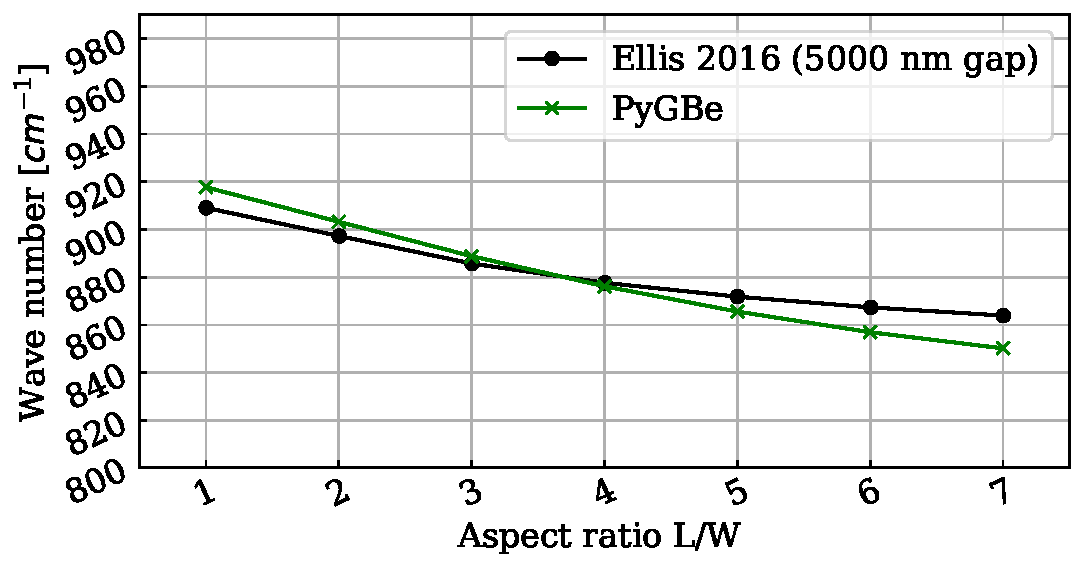
\includegraphics[width=0.85\textwidth]{AR_rep_FS4_Ellis2016.pdf} 
    \caption{Replication of figure S4 in the supplementary materials of Ellis et al., 2016. Wave
    number at which the $E^{\parallel}_{100}$ mode happens for different aspect ratios.}
    \label{fig:rep_FS4_ellis}
 \end{figure}
 
 \begin{table}
    \centering
    \caption{Percentage error for different aspect ratios.} 
    \label{tab:err_AR}
    \begin{tabular}{c c}
    \hline%\toprule
    AR & \% error \\
    \hline%\midrule
     $1$ & $0.95$ \\
     $2$ & $0.67$ \\
     $3$ & $0.35$ \\
     $4$ & $0.16$ \\
     $5$ & $0.72$ \\
     $6$ & $1.20$ \\
     $7$ & $1.59$ \\
    \hline%\bottomrule
    \end{tabular}
\end{table}

\subsection{Validation of \pygbe against experimental results in Fig. 2a of Ellis et al., and replications
of the corresponding computations}\label{ssec:validation}

The geometry used in the results of Figure 2a of Ellis et al. correspond to the case of aspect ratio $AR=4$. For this case,
we have the mesh provided by the authors. Since our computation for the mode $E^{\parallel}_{100}$ compares well with 
their results (percentage error of $0.16\%$), we chose this particular result from Ellis et al. to validate our simulations 
with their experimental results (red curve on their paper), as well as to replicate its corresponding computations (green 
curve on their paper). Figure 2a of Ellis et al. shows experimental and computational results of the reflectance of SiC pillar 
arrays with a gap of 500 nm, where the angle of incidence is 22$^\circ$ off-normal and the incoming polarization is parallel 
to the length of the pillar. Using \pygbe, we computed the extinction cross section of an isolated SiC pillar of aspect ratio
$AR=4$ with no substrate, submerged in air and under a constant electric field in the $z$-direction. The geometry was rotated to match
the angle of incidence of 22$^\circ$ used by Ellis et al. (see Figure \ref{fig:ellis_ang_inc}). Figure \ref{fig:pygbe_vs_exp_2a} 
shows the comparison of our simulations and the experimental results of Ellis et al. We can observe a noticeable difference in between 
the wave numbers at which the peaks occur. This difference may be attributed to the fact that in their experimental setup the 
separation between the pillars is $500$ nm, which implies there are coupling effects that are not considered in our simulations.

\begin{figure}
    \centering
    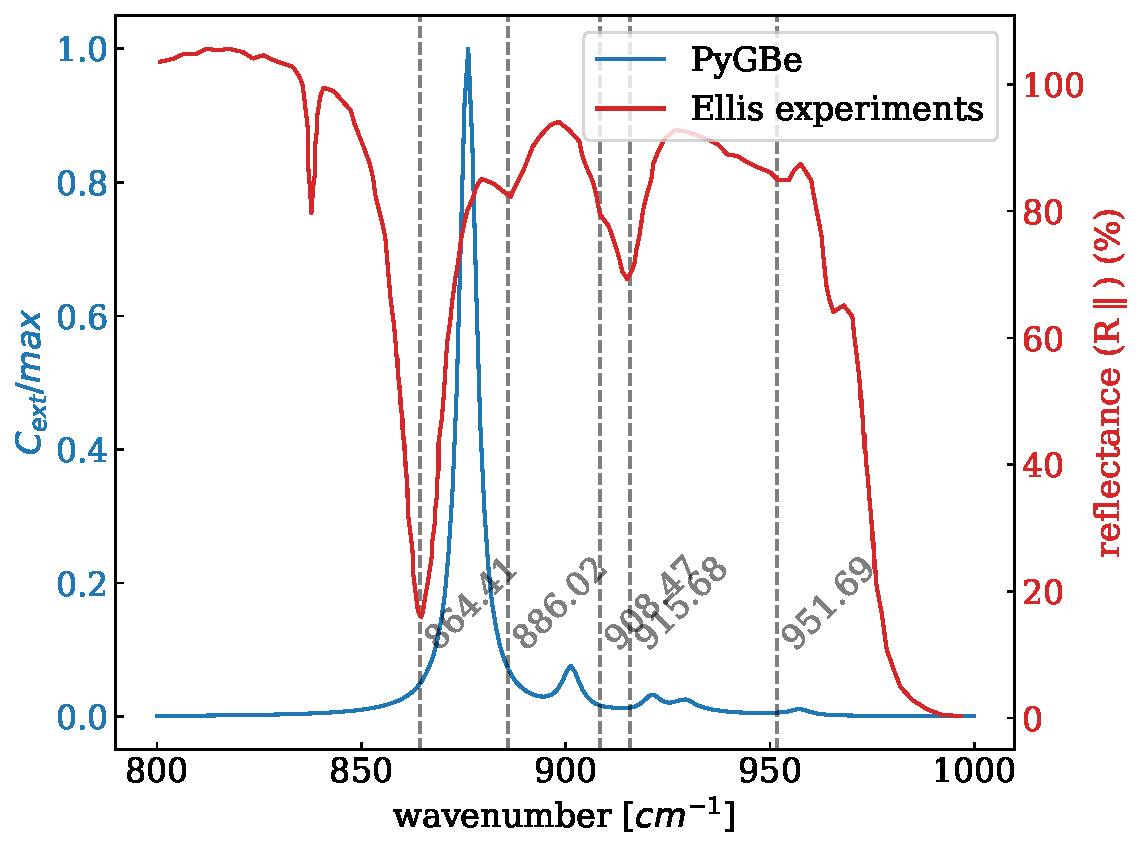
\includegraphics[width=0.85\textwidth]{pygbe_vs_exp_fig2a_Ellis.pdf} 
    \caption{\pygbe vs.\ the experiments presented in Figure 2a of Ellis et al., 2016 (we obtained the data 
    digitizing by hand from their figure using WebPlotDigitizer).}
    \label{fig:pygbe_vs_exp_2a}
 \end{figure}

\textbf{First-order correction.} 

Since our simulations are performed on an isolated prism and do not take into account the coupling effects 
in an array of prisms, we cannot strictly match the conditions to validate our solver. However, from Figure S4 in the supplementary material of 
Ellis et al., we know that this coupling effect affects the $E^{\parallel}_{100}$ mode by a shift of 12.17 cm$^{-1}$. Then, as a 
\textbf{first-order correction}, we can subtract this amount from our computations to account for the coupling effects. Figure \ref{fig:val_2a}, 
shows the results after applying the correction. It is worth mentioning that the peaks at 837 cm$^{-1}$ and 964 cm$^{-1}$ in the results of Ellis et al., 
are associated with the zone-folded LO (longitudinal) phonons of 4H-SiC, an effect they say to be beyond the scope of their analysis \cite{ellis2016}. Their 
analysis concentrates on the peaks that occur between 864 cm$^{-1}$ and 961 cm$^{-1}$. 
Figure \ref{fig:rep_2a} shows the comparison between the simulation results of Ellis et al. on Figure 2a of their paper (green curve), and our computations
after applying the first-order correction.

\begin{figure}
    \centering
    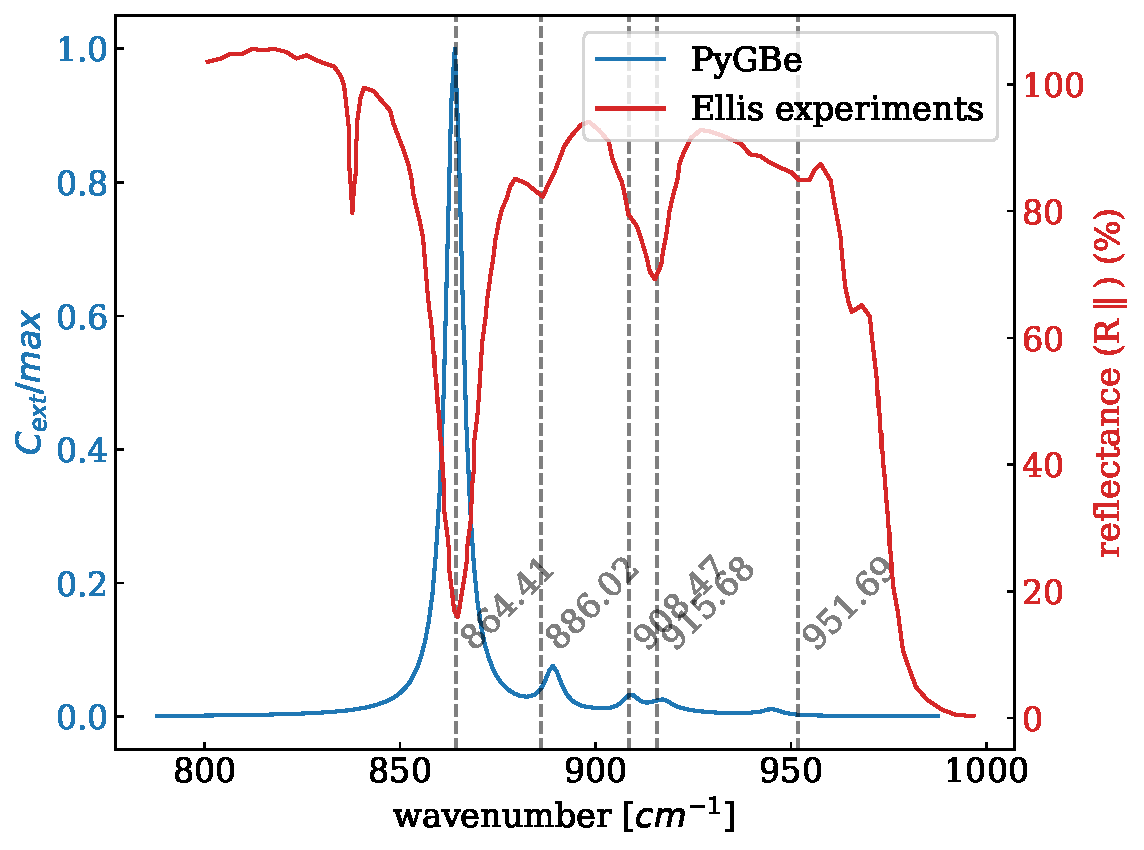
\includegraphics[width=0.85\textwidth]{validation_FOA_fig2a_Ellis.pdf} 
    \caption{Validation against experiments in Figure 2a of Ellis, et al., 2016, using the first-order correction, as explained in the text.}
    \label{fig:val_2a}
 \end{figure}

\begin{figure}
    \centering
    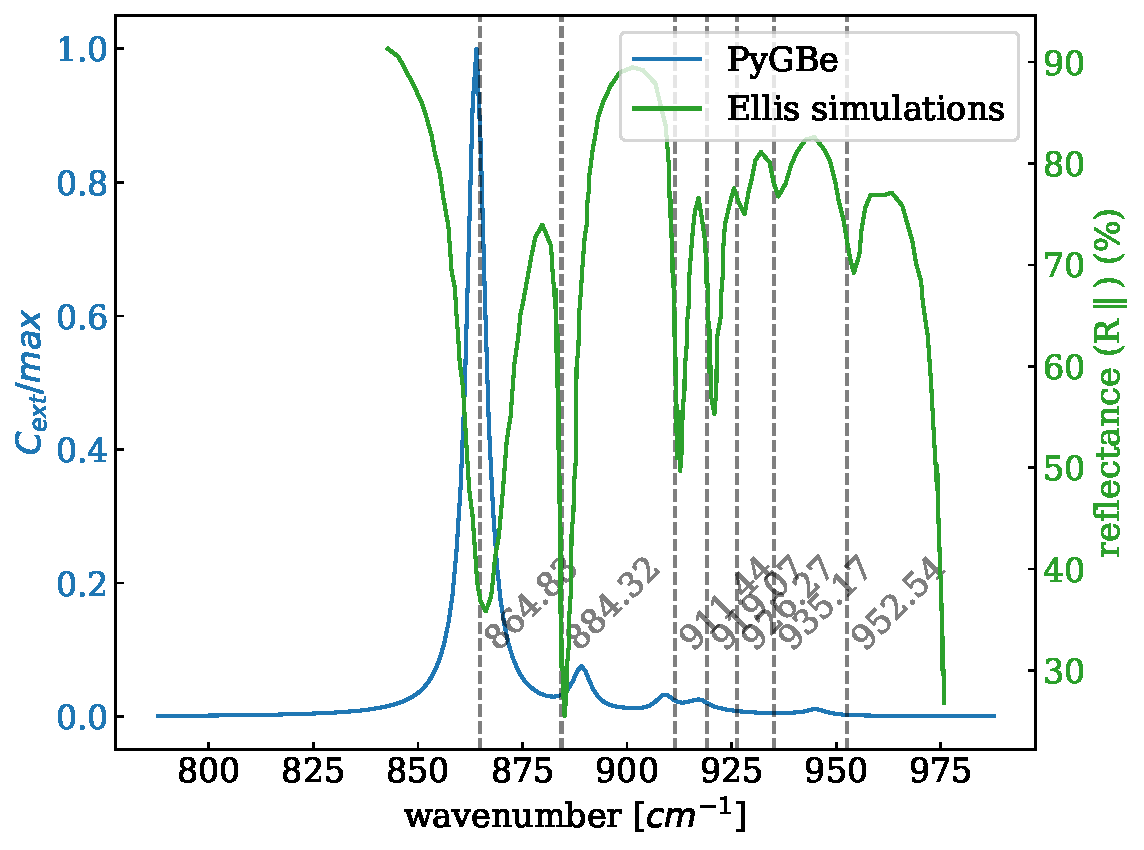
\includegraphics[width=0.85\textwidth]{replication_FOA_fig2a_Ellis.pdf} 
    \caption{Replication of the simulations in Figure 2a of Ellis et al., 2016, using the first-order correction, as explained in the text.}
    \label{fig:rep_2a}
 \end{figure}


In this section, we describe our attempt to replicate two results from Ellis et al. \cite{ellis2016} where they studied the effect of aspect ratio on the 
excitation of high-order modes in localized surface phonon-polariton nanostructures. Figure \ref{fig:rep_FS4_ellis} shows the results for
the replication of the black curve of Figure S4 of their supplementary material, where the relative errors between our computations and 
theirs is always smaller than 2$\%$. This replication study gave us the confidence to approach the replication of Figure 2a of Ellis et al., 
given that in that case they use a geometry with aspect ratio $AR=4$ presented the smallest error (see Table \ref{tab:err_AR}). Since 
Figure 2a of Ellis et al. shows results of experiments and simulations with the commercial software COMSOL, we not only pursued replication 
but we also sought the validation of \pygbe using these experimental results. The quantity plotted in the original figures is reflectance as a 
function of wavenumber, while we compute the extinction cross section. Since the quantity of interest is the wavenumber at which the resonance 
peaks/dips happen, the results are comparable. 

Figure \ref{fig:pygbe_vs_exp_2a} shows the results of our simulations using \pygbe on an isolated pillar, compared with the experimental results
of Ellis et al.\ on an array of pillars. The results with \pygbe do not account for the effect of coupling among the pillars, which explains the  
discrepancy on the wavenumbers at which the peaks occur. It is worth mentioning that we did not have the original data behind the plots of 
Ellis et al. therefore, we digitized the curves using the WebPlotDigitizer(\url{https://apps.automeris.io/wpd/}). Based on the results reported 
on Figure S4 of Ellis et al.\ for the $AR=4$ case, we proposed a first order correction that subtracts the shift on the wave number due to
coupling is of 12.17 cm$^{-1}$ (difference between black and red curves for $AR=4$ on figure S4 of the supplementary materials). Figure \ref{fig:val_2a}
and Figure \ref{fig:rep_2a} show the comparison of our corrected results with their experiments and simulations, respectively. We observe a good match 
of the wavenumber for the lower (and stronger) mode, as well as a good match for the third and fourth peaks. The wave number of the second peak, related 
to a longitudinal excitation (mode $L_{000}$ in Ellis et al.), presents a discrepancy that we believe is related to the fact that our 
pillar does not have a substrate underneath. The remaining (fifth) peak also presents a discrepancy, but in this case we could not identify the reason.
We did not analyze the peaks out of the range 864--961 cm$^{-1}$, since Ellis et al.\ describe these peaks to be associated with 
zone-folded LO (longitudinal) phonons of 4H-SiC, and outside the scope of their study.
After considering all these details, we can say that we have validated our solver \pygbe against the experimental results of 
Figure 2a, as well as replicated their computational results.

\section{Reproducibility and data management} \label{sec:repro_val}
 
All the results of this chapter have been accepted for publication in the journal 
Philosophical Transactions A \cite{ClementiBarba2020} and can be reproduced and replicated. \pygbe is openly developed and 
shared under the BSD3-clause license via its repository at \url{https://github.com/pygbe/pygbe}.

All results of this chapter were obtained on a lab workstation, built from parts. Hardware specifications are as follows:

\begin{itemize}
  \item CPU: Intel Core i7-5930K Haswell-E 6-Core 3.5GHz LGA 2011-v3
  \item RAM: G.SKILL Ripjaws 4 series 32GB (4 x 8GB)
  \item GPU: Nvidia Tesla K40c (with 12 GB memory)
\end{itemize}

Readers can reproduce all the figures in this chapter using the repro-packs shared in Zenodo. They include 
data and scripts needed to run the calculations reported in this chapter, the manually digitized data from the figures
in the source articles for our replication cases, as well as Jupyter notebooks with all the plotting code:

\begin{itemize}

\item[$\triangleright$] The problem datasets for replication of Rockstuhl et al., 2005, are in the manuscript repository, but also archived in Zenodo  at \href{https://doi.org/10.5281/zenodo.3962534}{10.5281/zenodo.3962534}  \cite{ClementiBarba2020-Zen_a}.

\item[$\triangleright$] Execution files for all runs are archived in Zenodo at \href{https://doi.org/10.5281/zenodo.3962576}{10.5281/zenodo.3962576} \cite{ClementiBarba2020-Zen_b}.

\item[$\triangleright$] The problem datasets for validation and replication of results from Ellis et al., 2016 are archived in Zenodo at \href{https://doi.org/10.5281/zenodo.3962584}{10.5281/zenodo.3962584}\cite{ClementiBarba2020-Zen_c}.

\item[$\triangleright$] The file sets for reproducing the figures for the replication of results from Rockstuhl et al., 2005 are archived in Zenodo at \href{https://doi.org/10.5281/zenodo.3962791}{10.5281/zenodo.3962791} \cite{ClementiBarba2020-Zen_d}.

\item[$\triangleright$] The file sets for reproducing the figures for the validation and replication of results from Ellis et al., 2017 are archived in Zenodo at \href{https://doi.org/3962797/zenodo.3962797}{10.5281/zenodo.3962797} \cite{ClementiBarba2020-Zen_e}.

\end{itemize}
